\section{Limits of Agreement}
% introduces
A third element of the Bland-Altman methodology, an interval known
as `limits of agreement' is introduced in \citet*{BA86}
(sometimes referred to in literature as 95\% limits of agreement).
Limits of agreement are used to assess whether the two methods of
measurement can be used interchangeably. \citet{BA86} refer to
this as the `equivalence' of two measurement methods. The specific purpose of the limits of
agreement must be
established clearly. \citet*{BA95} comment that the limits of agreement `how
far apart measurements by the two methods were likely to be for
most individuals', a definition echoed in their 1999 paper:

\begin{quote}"We can then say that nearly all pairs
of measurements by the two methods will be closer together than
these extreme values, which we call 95\% limits of agreement.
These values define the range within which most differences
between measurements by the two methods will lie."
\end{quote}

The limits of agreement (LoA) are computed by the following
formula:
\[
LoA = \bar{d} \pm 1.96 s_{d}
\]
with $\bar{d}$ as the estimate of the inter method bias, $s_{d}$
as the standard deviation of the differences and 1.96 is the 95\%
quantile for the standard normal distribution. (Some accounts of
Bland-Altman plots use a multiple of 2 standard deviations instead
for simplicity.)

The limits of agreement methodology assumes a constant level of bias throughout the range of measurements. Importantly the authors recommend prior determination of what would and would constitute acceptable
agreement, and that sample sizes should be predetermined to give an accurate conclusion. However \citet{mantha} highlights inadequacies in the correct application of limits of agreement, resulting in contradictory estimates limits of agreement in various papers.

\begin{quote}
``How far apart measurements can be without causing difficulties
will be a question of judgment. Ideally, it should be defined in
advance to help in the interpretation of the method comparison and
to choose the sample size \citep{BA86}".
\end{quote}


For the Grubbs `F vs C' comparison, these limits
of agreement are calculated as -0.132 for the upper bound, and
-1.08 for the lower bound. Figure 1.9 shows the resultant
Bland-Altman plot, with the limits of agreement shown in dashed
lines.


\begin{figure}[h!]
\begin{center}
  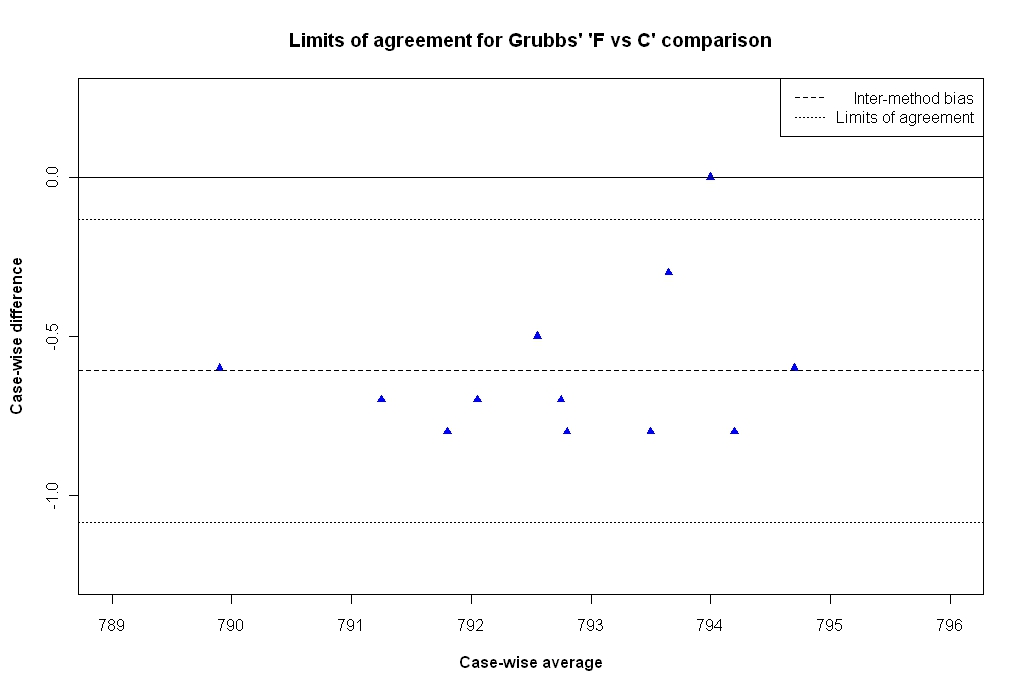
\includegraphics[width=125mm]{GrubbsBAplot-LOA.jpeg}
  \caption{Bland-Altman plot with limits of agreement}\label{GrubbsBAplot-noLOA}
\end{center}
\end{figure}

%But as \citet*{BA86} point out this may not be the case. Variants of the limits of agreement that overcome this
% problem shall be introduced in due course.


%-------------------------------------------------------------------------------%
\end{document}
